% Bibliografia
\printbibliography[heading=bibintoc]

% Appendixy
\begin{appendices}
\chapter{Zmodyfikowane prompty do C3}

\begin{minipage}{\linewidth}
\lstinputlisting[
caption=Zmodyfikowany prompt z \code{C3} służący do znalezienia istotnych tabel,
language=prompt,
escapechar=@,
label={lst:c3-table-recall-prompt}
]{listings/c3_table_recall.txt}
\end{minipage}

\begin{minipage}{\linewidth}
\lstinputlisting[
caption=Zmodyfikowany prompt z \code{C3} służący do znalezienia istotnych kolumn,
language=prompt,
escapechar=@,
label={lst:c3-column-recall-prompt}
]{listings/c3_column_recall.txt}
\end{minipage}

\begin{minipage}{\linewidth}
\lstinputlisting[
caption=Zmodyfikowany prompt z \code{C3} służący do generowania zapytania SQL,
language=prompt,
escapechar=@,
label={lst:c3-generate}
]{listings/c3_generate.txt}
\end{minipage}

\chapter{Interfejs graficzny}

\begin{figure}[ht!]
  \centering
  \fbox{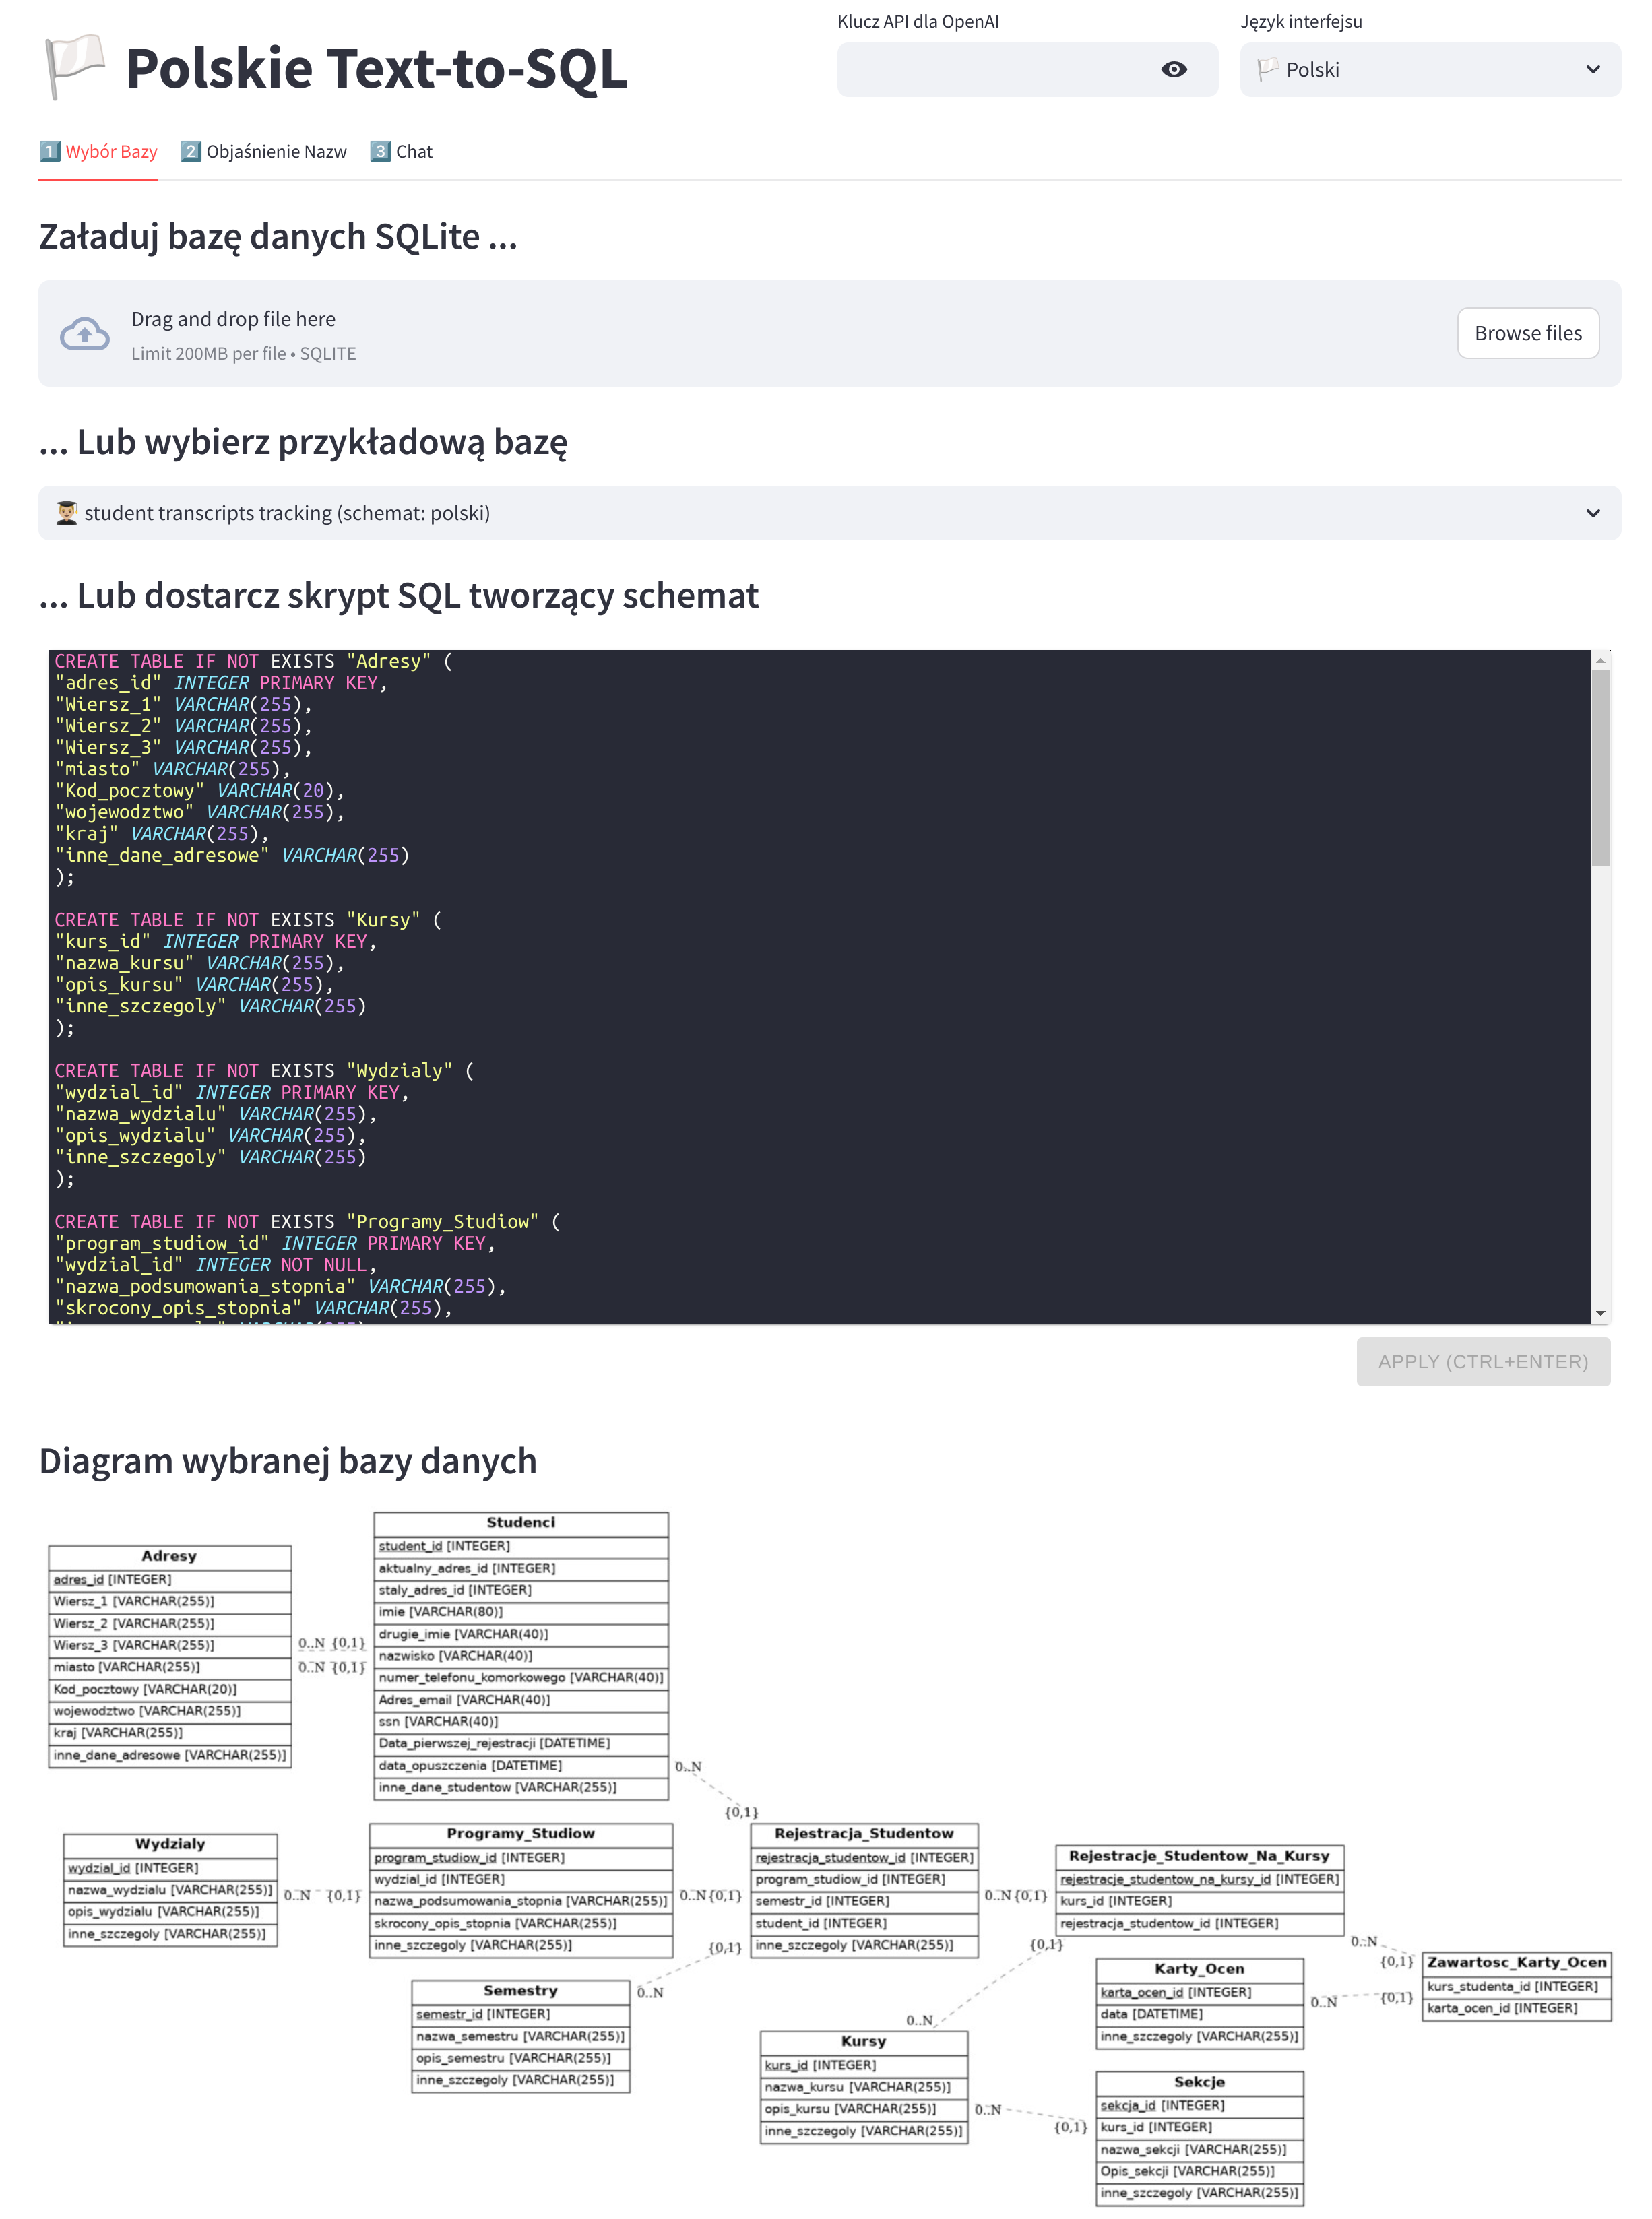
\includegraphics[width=1.0\linewidth]{images/gui_selection_tab.png}}
  \caption{Zakładka wyboru bazy danych w stworzonym interfejsie graficznym}
  \label{fig:gui-selection-tab}
\end{figure}

\begin{figure}[ht!]
  \centering
  \fbox{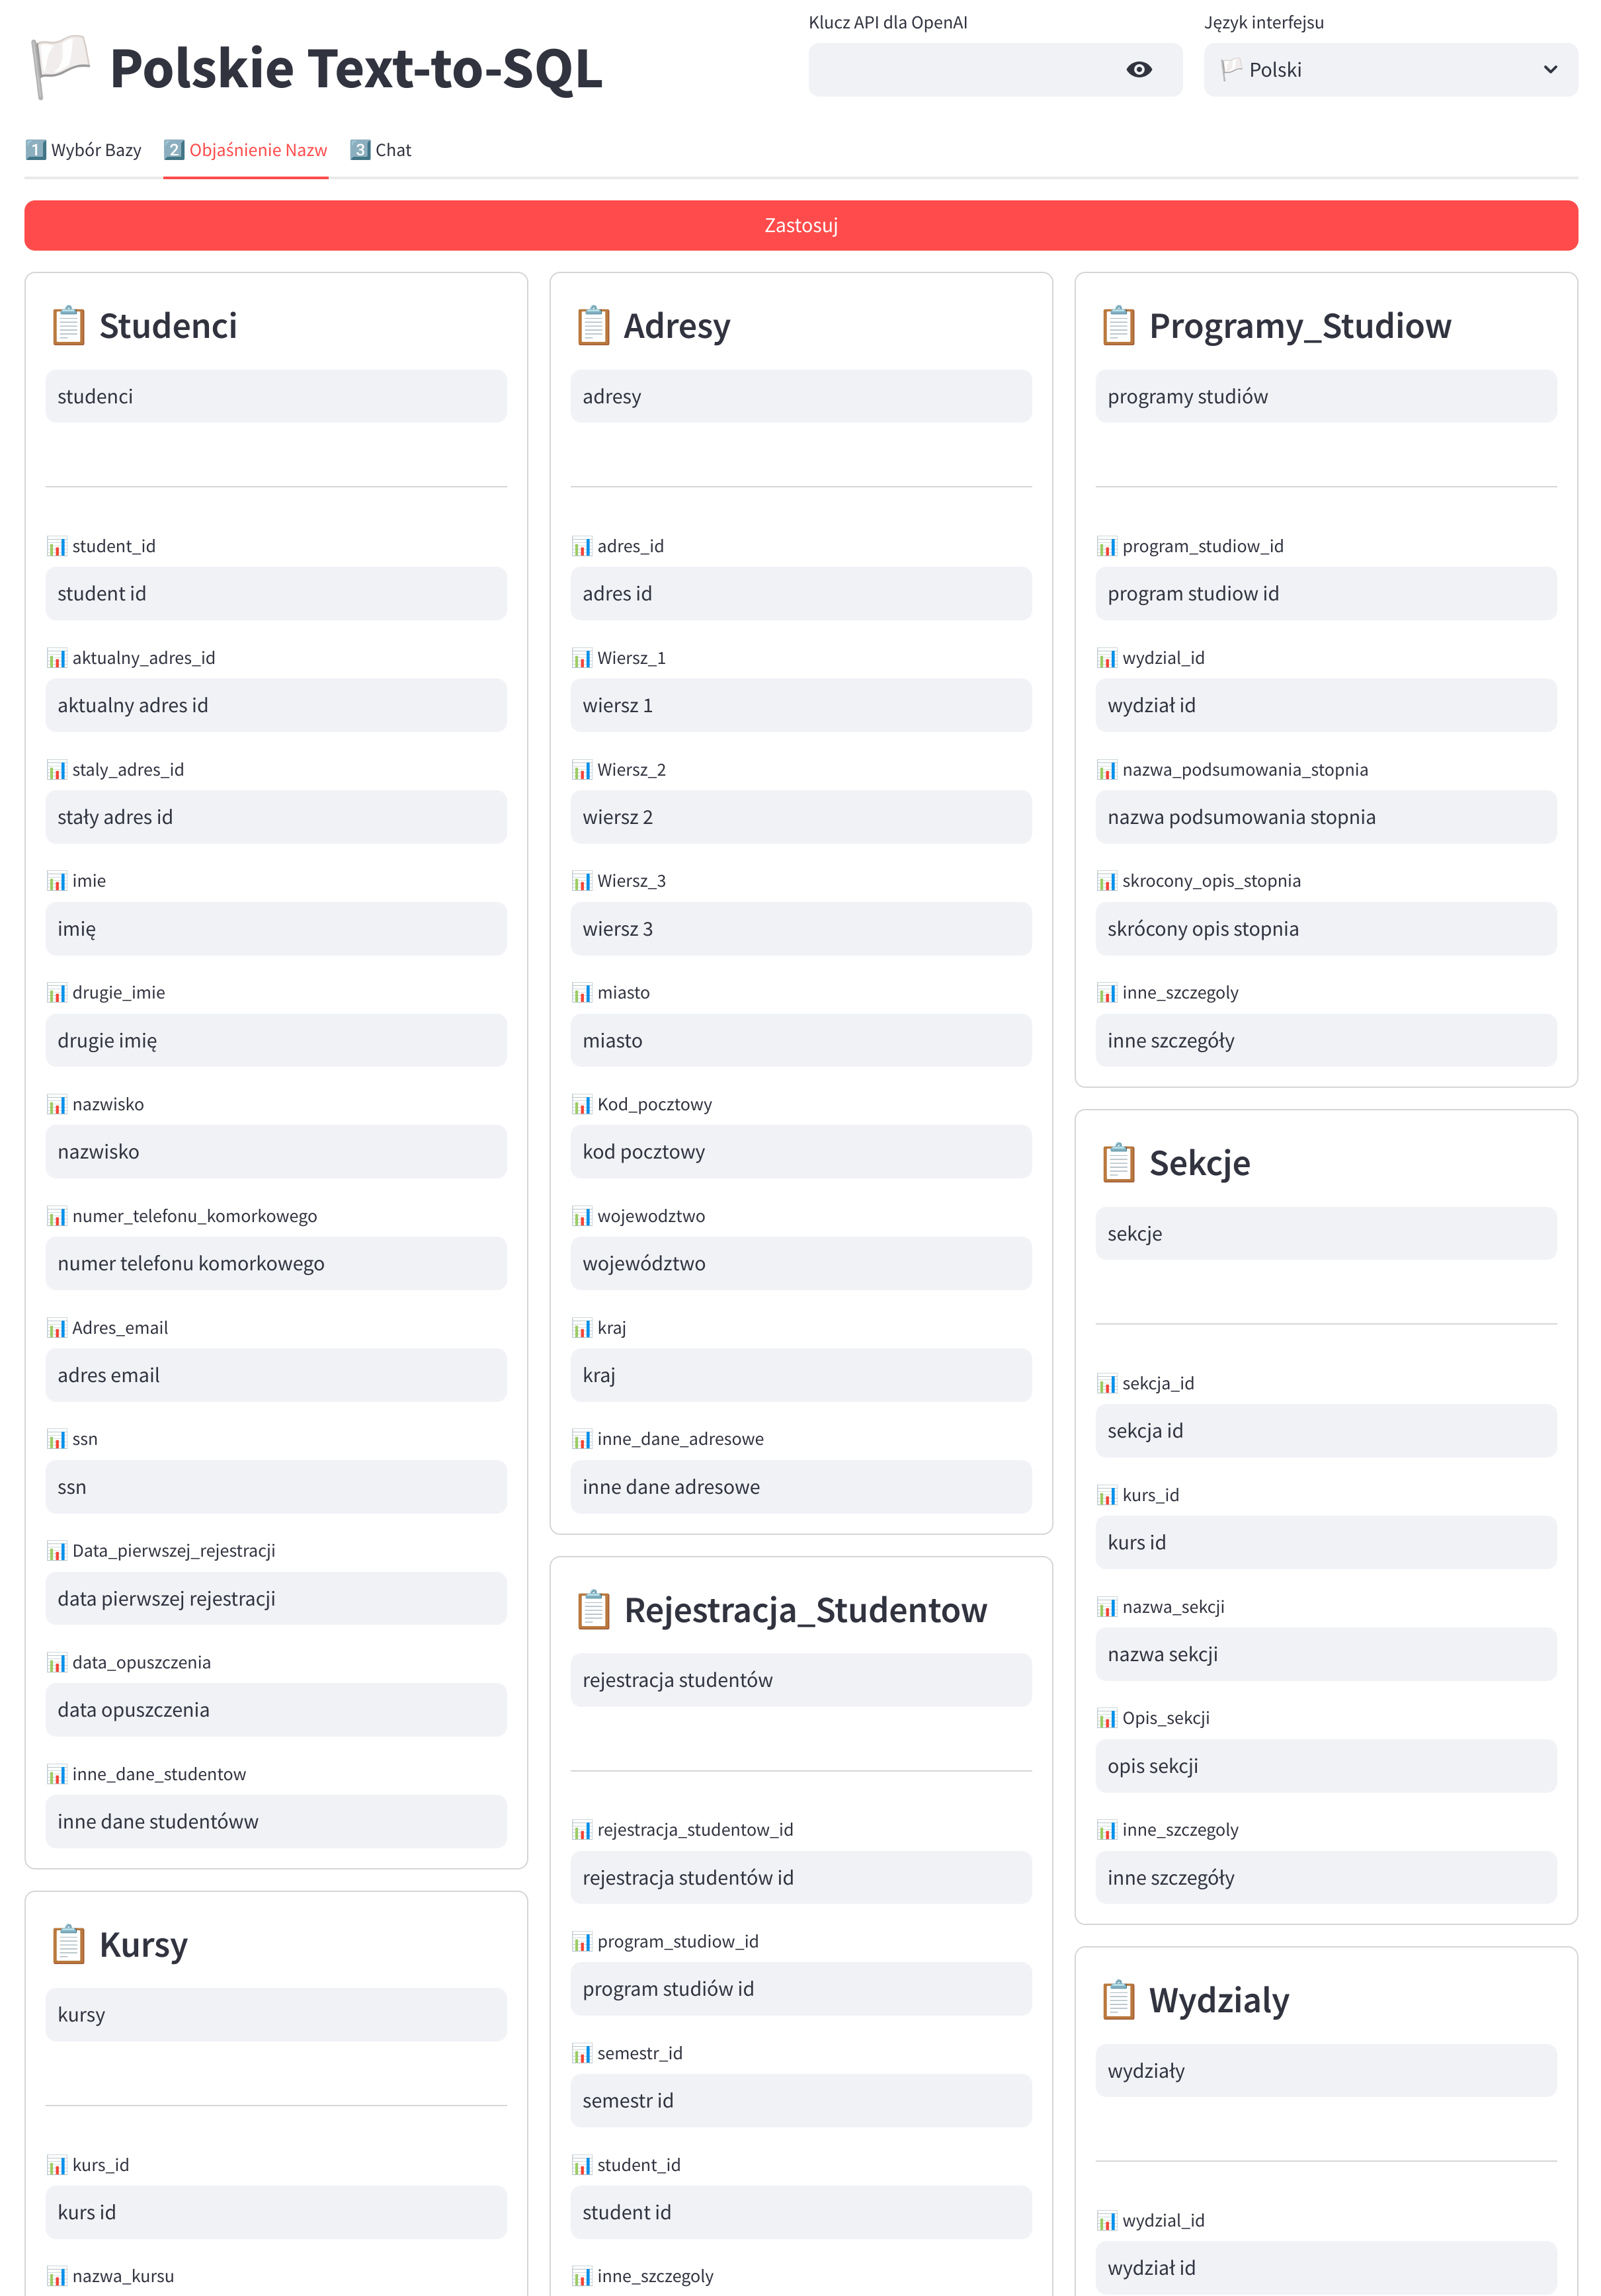
\includegraphics[width=1.0\linewidth]{images/gui_clarification_tab.png}}
  \caption{Zakładka objaśnienia nazw schematu w stworzonym interfejsie graficznym}
  \label{fig:gui-clarification-tab}
\end{figure}

\begin{figure}[ht!]
  \centering
  \fbox{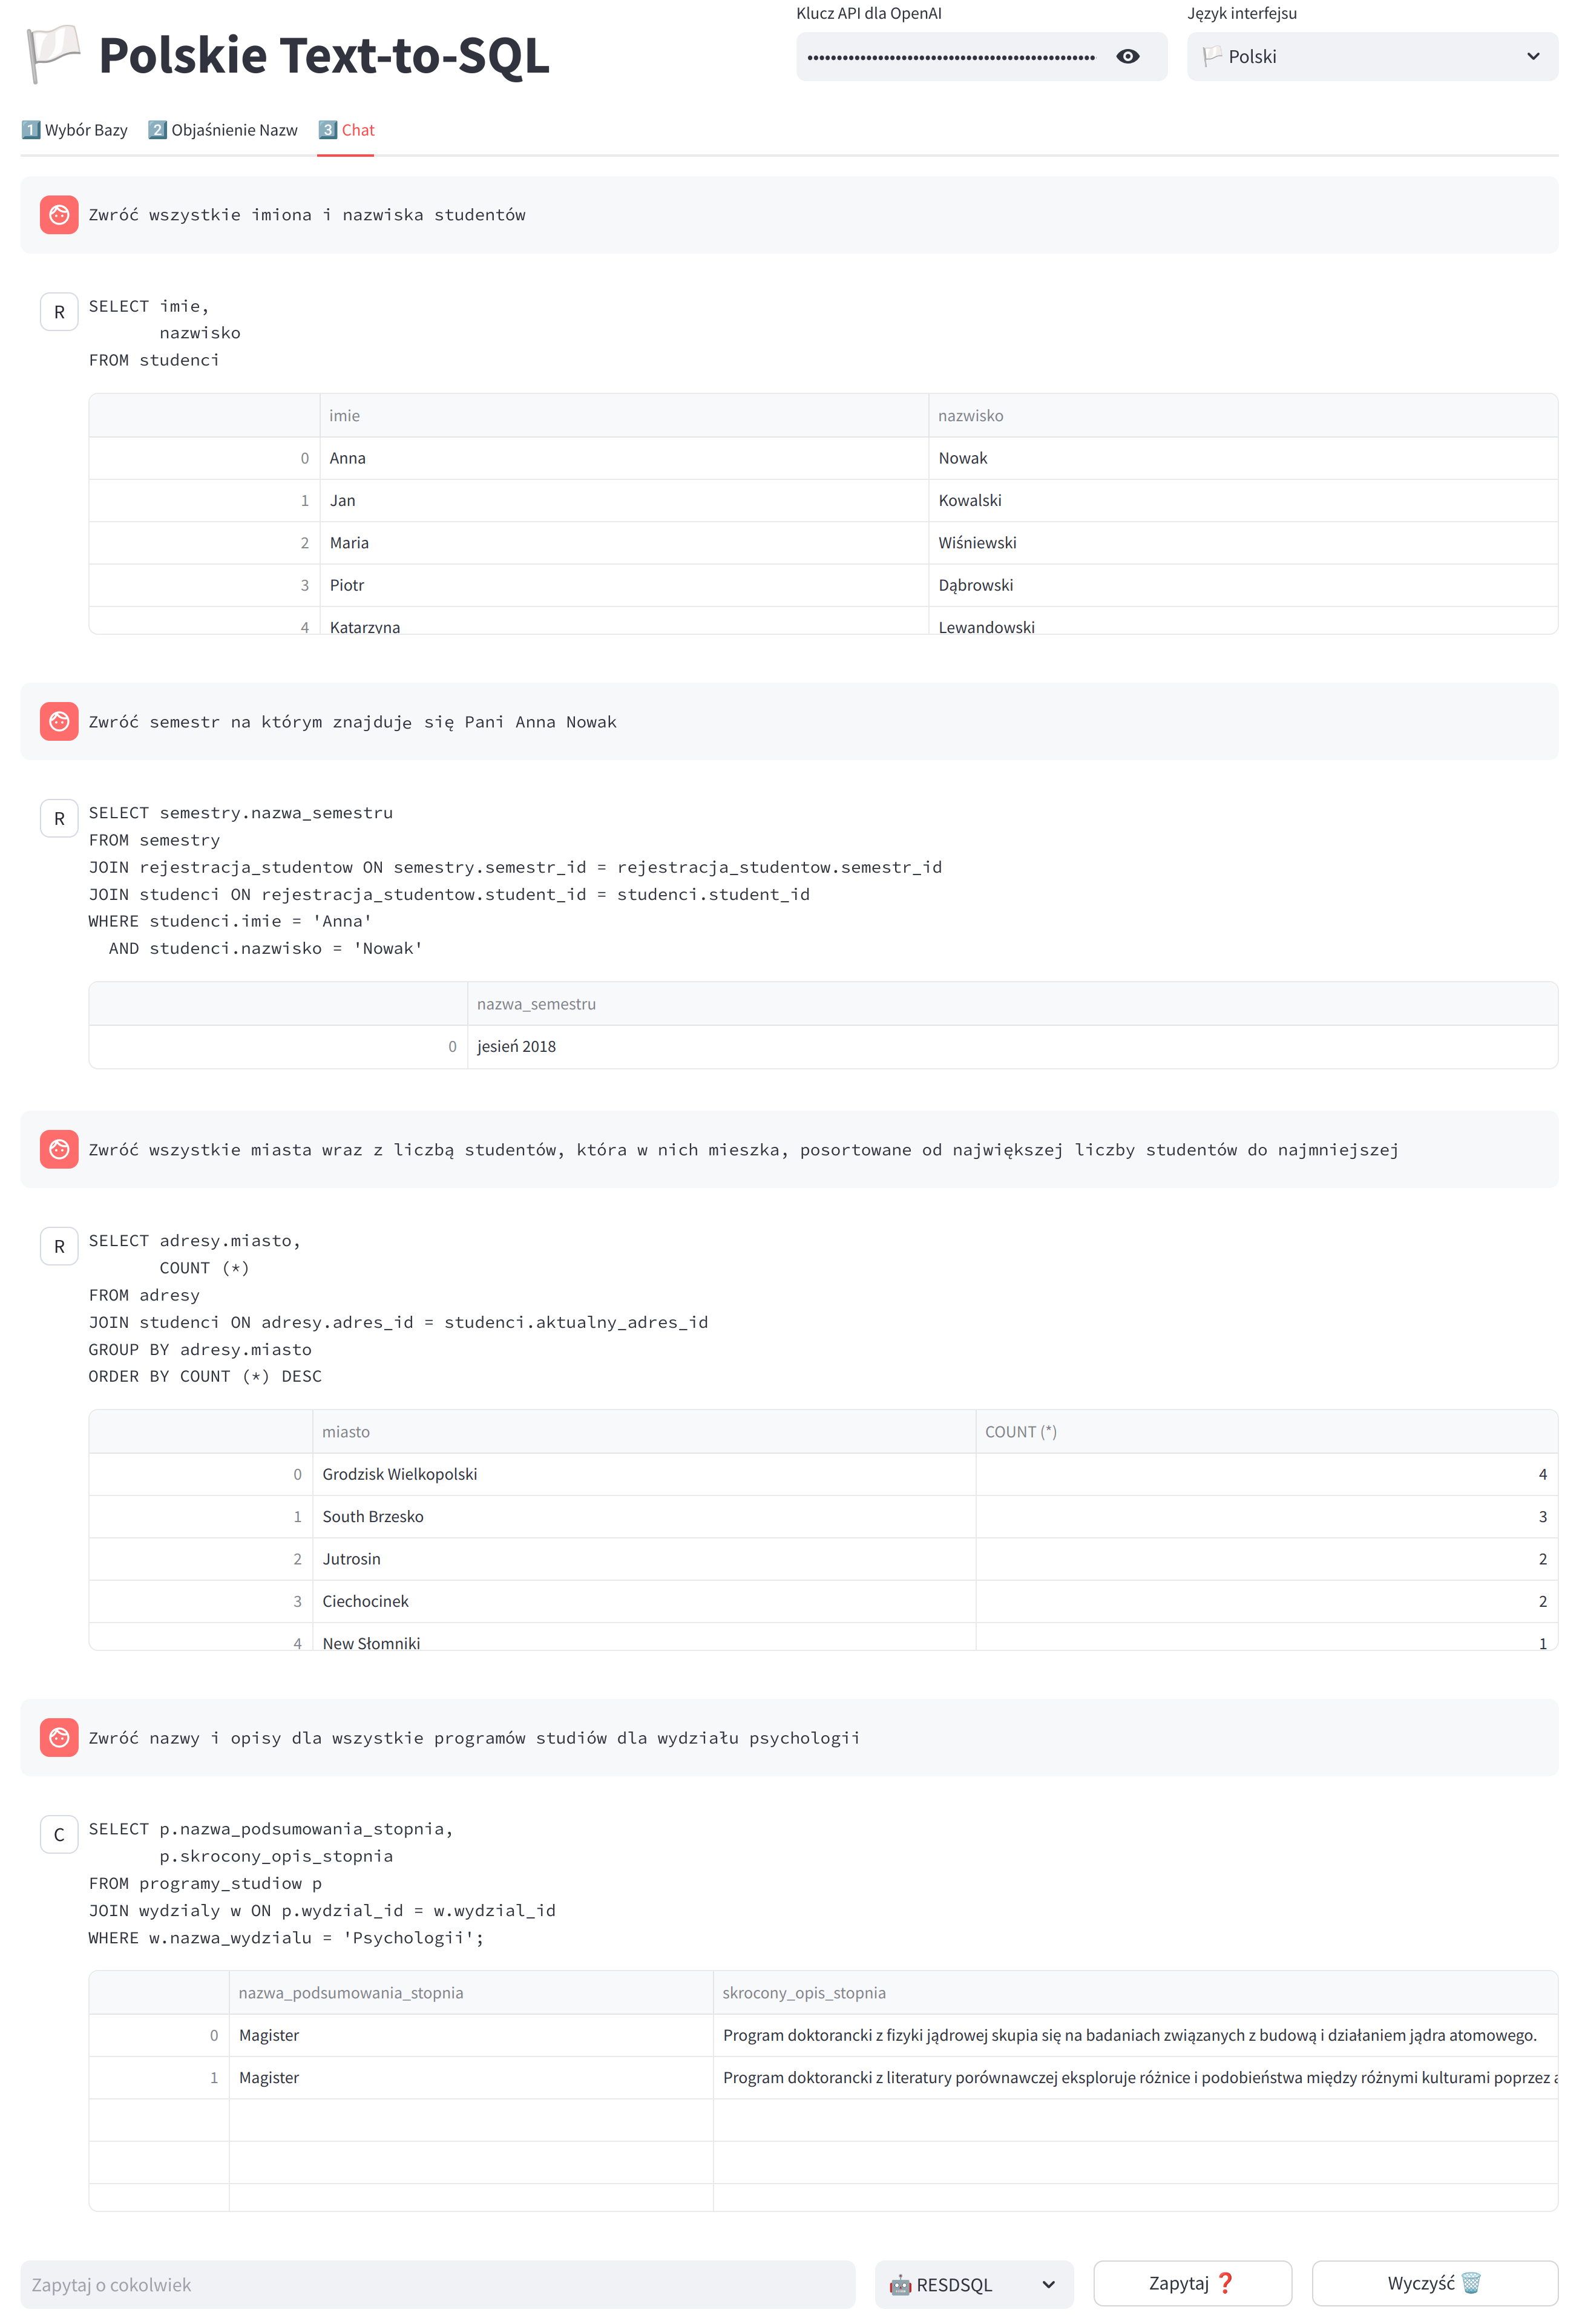
\includegraphics[width=1.0\linewidth]{images/gui_chat_tab.png}}
  \caption{Zakładka chatu w stworzonym interfejsie graficznym}
  \label{fig:gui-chat-tab}
\end{figure}

\end{appendices}

% Wykaz rysunków
\setstretch{1.400}
\newcommand{\loftitle}{Wykaz rysunków}
\clearpage
\chapter*{\loftitle}
\addcontentsline{toc}{chapter}{\loftitle}
\vspace{3mm}
\listoffigures
\setstretch{1.5}

% Wykaz tabel
\newcommand{\lottitle}{Wykaz tabel}
\clearpage
\chapter*{\lottitle}
\addcontentsline{toc}{chapter}{\lottitle}
\listoftables

% Wykaz listingów
\newcommand{\loltitle}{Wykaz listingów}
\clearpage
\chapter*{\loltitle}
\addcontentsline{toc}{chapter}{\loltitle}
\vspace{3mm}
\lstlistoflistings

% Wykaz skrótów
\newcommand{\lostitle}{Wykaz skrótów}
\clearpage
\chapter*{\lostitle}
\addcontentsline{toc}{chapter}{\lostitle}
\begin{itemize}
\abbrev{API}{Application Programming Interface}
\abbrev{AST}{Abstract Syntax Tree}
\abbrev{DK}{Domain Knowledge}
\abbrev{RAT}{Relation Aware Transformer}
\abbrev{SQL}{Structured Query Language}
\abbrev{JSON}{JavaScript Object Notation}
\abbrev{SSOT}{Single Source of Truth}
\abbrev{NER}{Named Entity Recognition}
\abbrev{ASCII}{American Standard Code for Information Interchange}
\abbrev{LSTM}{Long Short-Term Memory}
\abbrev{GPG}{GNU Privacy Guard}
\abbrev{HF}{Hugging Face}
\abbrev{AUC}{Area Under the ROC Curve}
\abbrev{VRAM}{Video Random Access Memory}
\end{itemize}
